% Please do not change the document class
\documentclass{scrartcl}

% Please do not change these packages
\usepackage[hidelinks]{hyperref}
\usepackage[none]{hyphenat}
\usepackage{setspace}
\usepackage{graphicx}
\usepackage{cite}
\usepackage[export]{adjustbox}
\doublespace

% You may add additional packages here
\usepackage{amsmath}

% Please include a clear, concise, and descriptive title
\title{Does scrum-orientated micro-versioning aid the scrum team track sprint goals in game development?}

% Please do not change the subtitle
\subtitle{COMP150 - Agile Development Practice}

% Please put your student number in the author field
\author{1700522}

\begin{document}

\maketitle

\abstract{Games development teams are constantly working on a number of features for the game simultaneously and often have multiple methods that they can take to complete these goals. Within agile development the use of the scrum framework and sprints ties into the use of micro-versioning, which allows the development team to make use of tools in version control within the framework to develop these separate features or alternative approaches simultaneously and in isolation from each other to be merged into the main version. It is the position of this paper that the use of this technique will aid the team in tracking their goals through each goal possessing its own micro-version.}

\section{Introduction}
Within the games development industry a number of software development practices are in use, one of these known as Agile has a number of advantages for creative projects and as such has been adopted successfully in the industy \cite{AgileGameDevelopmentCKeith}. With the adaptability of agile in mind it is the view of this paper that the use of micro-versioning aids the game development team with meeting their goals. This is through the ability to make use of simultaneous development and the ability for experimental development without jeopardizing the main project.

\section{How does micro-versioning link to agile development?}
Within the agile manifesto there are 12 principles and the 12th of these is ``At regular intervals, the team reflects on how 
to become more effective, then tunes and adjusts 
its behavior accordingly.''\cite{AgileManifesto} This particular point on the agile manifesto is usually done using sprints\cite{AdoptingScrum}. The use of micro-versioning within SCRUM can be used to track the goals of a sprint. Micro-versions can be defined as the use of version control operations that can be used within experimentation and development of features\cite{mikami2017micro}.

\begin{figure}[h!]
	\begin{center}
	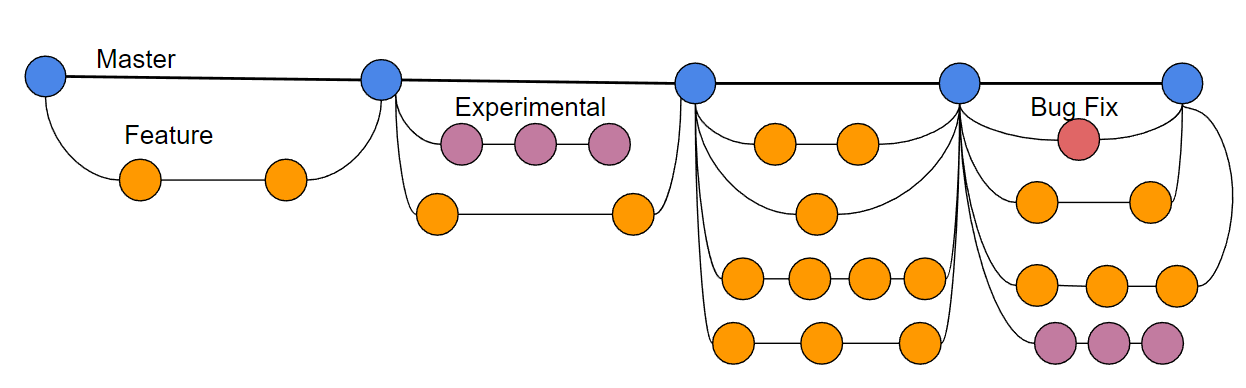
\includegraphics [width=0.79\textwidth,inner]{Micro-VersioningExampleDiagram}
	\caption{A diagram of micro-versioning through branching}
	\label{MicroVersioningDiagram}
	\end{center}
\end{figure}

Figure \ref{MicroVersioningDiagram} shows the implementation  of micro-versioning through a technique in version control known as branching. Branching is a technique in version control systems that enables the creation of multiple versions under the main version, (defined above as micro-versions)\cite{chacon2014pro}. During a sprint the user stories that are used as sprint goals will not necessarily be done by the same developer and as such need to be simultaneously developed. In these scenarios small scale version control can be used in branches to attempt to avoid clashes that will need to be resolved in version control. In an alternative scenario there could be multiple ways of completing the same task within a game and as such micro-versions can be used to experiment with these methods.


\section{How does micro-versioning aid in video game development?}
Polan{\v{c}}e{\'c} and Mekterovi{\'c} set out the stages of developing a MOBA in the context of the Unity engine. \cite{polanvcec2017developing} While they do not go into a great deal of detail it can be seen that these factors that can easily be simultaneously developed to increase the speed and efficiency of the development team. For each of these features or an experiment as to how to implement a feature. In 2011 an investigation into version control practices at the University of Calgary \cite{phillips2011branching}.
	\begin{center}
	
	\begin{tabular}{ c c }
		Table 1: & Branch Types Created \cite{phillips2011branching} \\
		\hline
 		Branch Type & Number of Respondents   \\ 
 		\hline
 		Release & 93 (73\%)   \\  
 		Experiment/Prototype & 90 (70\%)\\  
 		Feature & 82 (64\%)     \\  
 		Bug Fix & 53 (41\%)     \\  
 		Contributor (Personal) & 46 (36\%)     \\  
 		Merge & 37 (29\%)     \\  
 		Tool/Utility & 18 (14\%)     \\  
 		Platform/SKU &  16 (13\%)  \\
 		\hline     
	\end{tabular}

	\end{center}
As can be seen in table 1 branching is commonly used in both experimentation and feature development both having over 80\% of respondents. Both of these uses are forms of micro-versioning and while this is in software development practices the same methodologies can be applied to programming in video games. With the creative thinking involved in video games it is likely that there will be a large number of possible, thought of solutions to a single problem. In a typical context only one of these would progress forwards into the sprint, but with the use of micro-versioning the programming team can be split. As such multiple solutions designed and tested as to find either the mechanically optimal one or the one that best suits the theme of the game. 

What people find to be the main issue with the use of micro-versioning and branching is the merging of these branches at the end. In response to this a model based on the GitWaterFlow was developed at Scality in France in 2016 \cite{GitWaterFlow}. With the use of other Gate keeping and merging bots in combination with integration bots the team at Scality managed to create an all purpose bot known as ``Bert-E'' that could manage these branches and avoid the issues that a number of developers have found with the micro-versioning model.
\begin{figure}[h!]
	\begin{center}
	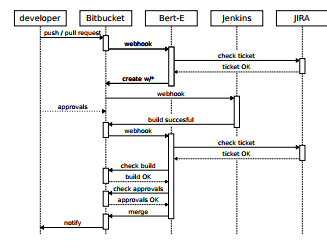
\includegraphics [width=0.79\textwidth,inner]{BertE}
	\caption{Merging a feature branch with Bert-E -Best case scenario \cite{GitWaterFlow}}
	\label{BertE}
	\end{center}
\end{figure}

Figure \ref{BertE}  shows how a bot can be used to sit between the humans using the version control system to manage the system and prevent clashes from occurring.
\section{The disadvantages of micro-versioning}
While this paper is in favour of micro-versioning it is not without problems. The use of branching without the addition of bots such as ``Bert-E'' can sometimes be difficult. In the investigation completed by the team at the University of Calgary one of their participants was quoted as saying ``We are a team of four senior developers (by
which I mean we’re all over 40 with 20+ years
each of development experience) and not one of
us has had a positive experience in the past with
branching the mainline...The branch is easy - it’s
the merge at the end that’s painful''\cite{phillips2011branching}. This is what appears to be the main issue with branching. The merging of all of these branches at the end can be problematic as the more branches there are the more likely it is that there will be a clash.
\begin{center}
	\begin{tabular}{c c c}
		\hline
		Table 2: Most Significant Merge Problem \cite{phillips2011branching} \\
		\hline
		Merge Problem & \# of & Respondents \\
		& All Projects & Large, Active \\
		\hline
		Merge Conflicts & 69(54\%) & 6(32\%) \\
		Other & 20(16\%) & 2(11\%) \\
		Test Regressions & 17(13\%) & 2(21\%)\\
		Cross-Cutting Regressions & 12(9\%) & 4(21\%) \\
		Loss of Productivity & 7(5\%) & 2(10\%) \\
		Compilation Errors & 3(2\%) & 1(5\%) \\
		\hline
	\end{tabular}
\end{center}
As can be seen in table 2 the main issue is merge conflicts, which was explored by Scality \cite{GitWaterFlow}. Among the issues was also a loss of productivity with 10\% of active participants having this issue, this is directly a loss of productivity caused by branch destabilisation and merge errors. This is the greatest weakness of the model as this disruption of work flow could result in more time needing to be dedicated to an already time and resource heavy method of development.
\section{Conclusion}

In conclusion the micro-versioning model has a clear place in video game design, especially in the context of programming as this is where the combination of experimental and feature development is. In the industry this approach can be utilised for everything from the development of control schemes to the creation and implementation of core mechanics. In addition to how the micro-versioning model can be used to develop experimental branches of the same feature it can also be used for the simultaneous development of multiple features of the game. This is done while keeping each isolated until they merge into the main branch. The main flaw in the micro-versioning model is the final merging at the end of the sprin\cite{phillips2011branching}. As has been found in the research at Scality has found is the use of bot software as to limit the number of clashes in the final merge\cite{GitWaterFlow}. 
\newpage
\bibliography{references}{}
\bibliographystyle{ieeetran}

\end{document}
